\section{k-Means Clustering}

\begin{frame}{From PCA to Clustering}
\begin{itemize}
  \item PCA reduced dimension by maximizing projected variance.
  \pause
  \item k-means keeps the same geometric setting, but changes the goal.
  \pause
  \item Now the task is to partition unlabeled examples into $k$ compact groups.
  \pause
  \item The key idea is still optimization.
\end{itemize}
\end{frame}

\begin{frame}{Clustering Task}
\begin{columns}[T]
\column{0.52\textwidth}
\begin{itemize}
  \item Input: examples $x_1,\dots,x_n \in \mathbb{R}^d$ with no target labels.
  \pause
  \item Output: a partition of the dataset into $k$ groups.
  \pause
  \item The result depends on the representation, the distance, and the chosen value of $k$.
\end{itemize}

\pause
\column{0.48\textwidth}
\textbf{Typical uses}
\begin{itemize}
  \item customer segmentation,
  \pause
  \item grouping embeddings or documents,
  \pause
  \item prototype compression,
  \pause
  \item exploratory analysis before downstream modeling.
\end{itemize}
\end{columns}

\pause
\begin{rlintuition}
PCA asks for informative directions. k-means asks for compact groups.
\end{rlintuition}
\end{frame}

\begin{frame}{Formal Setup}
\begin{itemize}
  \item Let $X=\{x_1,\dots,x_n\}$ with each $x_i \in \mathbb{R}^d$.
  \pause
  \item Fix the number of clusters $k$.
  \pause
  \item For each cluster $r \in \{1,\dots,k\}$, define a centroid $\mu_r \in \mathbb{R}^d$.
  \pause
  \item Each example receives an assignment $c_i \in \{1,\dots,k\}$.
  \pause
  \item Therefore the unknowns are both the assignments $c=(c_1,\dots,c_n)$ and the centroids $\mu=(\mu_1,\dots,\mu_k)$.
\end{itemize}
\end{frame}

\begin{frame}{The k-Means Objective}
\begin{itemize}
  \item k-means minimizes the within-cluster sum of squares:
  \begin{equation}
    J(c,\mu)
    =
    \sum_{r=1}^{k}\sum_{i:c_i=r}\|x_i-\mu_r\|_2^2.
    \label{eq:kmeans-objective}
  \end{equation}
  \pause
  \item A smaller value means that assigned points lie closer to their cluster centroid.
  \pause
  \item The method is therefore tied to squared Euclidean geometry.
\end{itemize}
\end{frame}

\begin{frame}{Assignment Step}
\begin{itemize}
  \item Suppose the centroids $\mu_1,\dots,\mu_k$ are fixed.
  \pause
  \item Then the best assignment for each example is the nearest centroid:
  \begin{equation}
    c_i
    =
    \arg\min_{r \in \{1,\dots,k\}}
    \|x_i-\mu_r\|_2^2.
    \label{eq:kmeans-assignment}
  \end{equation}
  \pause
  \item This is the same distance computation idea already used in k-NN.
  \pause
  \item The difference is that here there are no labels, only centroids.
\end{itemize}
\end{frame}

\begin{frame}{Why the Update Step Uses the Mean}
\begin{itemize}
  \item Now fix the assignments and optimize one centroid $\mu_r$.
  \pause
  \item The cluster-specific objective is
  \begin{equation}
    J_r(\mu_r)=\sum_{i:c_i=r}\|x_i-\mu_r\|_2^2.
    \label{eq:cluster-objective}
  \end{equation}
  \pause
  \item Setting the gradient to zero gives
  \begin{equation}
    \nabla_{\mu_r}J_r(\mu_r)
    =
    -2\sum_{i:c_i=r}(x_i-\mu_r)=0.
    \label{eq:cluster-gradient}
  \end{equation}
  \pause
  \item Therefore
  \begin{equation}
    \mu_r
    =
    \frac{1}{|\{i:c_i=r\}|}
    \sum_{i:c_i=r}x_i.
    \label{eq:centroid-mean}
  \end{equation}
  \pause
  \item So the best centroid is the arithmetic mean of the assigned examples.
\end{itemize}
\end{frame}

\begin{frame}{Graphic: One Full Iteration}
\centering
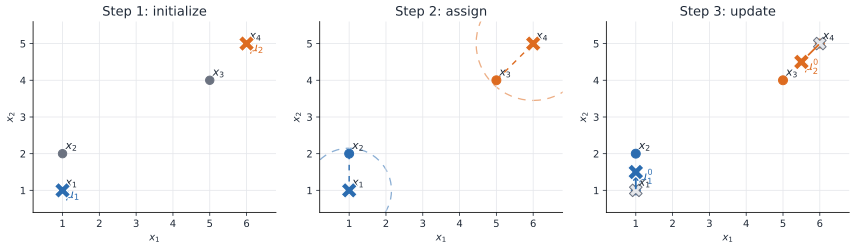
\includegraphics[width=0.97\textwidth]{figures/kmeans/kmeans_iteration_panels.pdf}

\vspace{0.35em}
\begin{itemize}
  \item The method alternates between nearest-centroid assignment and mean update.
  \pause
  \item This is the whole computational core of k-means.
\end{itemize}
\end{frame}

\begin{frame}{Worked Numerical Example}
\small
\begin{itemize}
  \item Let
  \[
    x_1=(1,1),\quad x_2=(1,2),\quad x_3=(5,4),\quad x_4=(6,5),
  \]
  with initial centroids $\mu_1=(1,1)$ and $\mu_2=(6,5)$.
  \pause
  \item For $x_2$,
  \[
    \|x_2-\mu_1\|_2^2 = 1,\qquad
    \|x_2-\mu_2\|_2^2 = 34,
  \]
  so $x_2$ goes to cluster $1$.
  \pause
  \item For $x_3$,
  \[
    \|x_3-\mu_1\|_2^2 = 25,\qquad
    \|x_3-\mu_2\|_2^2 = 2,
  \]
  so $x_3$ goes to cluster $2$.
  \pause
  \item Hence
  \[
    c_1=c_2=1,\qquad c_3=c_4=2,
  \]
\end{itemize}
\end{frame}

\begin{frame}{Worked Numerical Example: Update}
\small
\begin{itemize}
  \item From
  \[
    c_1=c_2=1,\qquad c_3=c_4=2,
  \]
  the updated centroids are
  \[
    \mu_1'=\frac{x_1+x_2}{2}=(1,1.5),\qquad
    \mu_2'=\frac{x_3+x_4}{2}=(5.5,4.5).
  \]
  \pause
  \item The objective decreases from $J=3$ to $J=1.5$ after the update.
\end{itemize}
\end{frame}

\begin{frame}{Alternating Optimization}
\begin{itemize}
  \item k-means repeats two exact partial optimizations:
  \pause
  \item \textbf{Assignment step:} minimize \eqref{eq:kmeans-objective} over $c$ with fixed $\mu$.
  \pause
  \item \textbf{Update step:} minimize \eqref{eq:kmeans-objective} over $\mu$ with fixed $c$.
  \pause
  \item Therefore each step does not increase the objective.
  \pause
  \item The objective decreases until the assignments stop changing.
\end{itemize}
\end{frame}

\begin{frame}{Basic k-Means Algorithm}
\begin{enumerate}
  \item Choose initial centroids $\mu_1,\dots,\mu_k$.
  \pause
  \item Assign each example to its nearest centroid.
  \pause
  \item Replace each centroid by the mean of its assigned examples.
  \pause
  \item Repeat until the assignments stop changing or the objective changes very little.
\end{enumerate}
\end{frame}

\begin{frame}{Initialization Sensitivity}
\centering
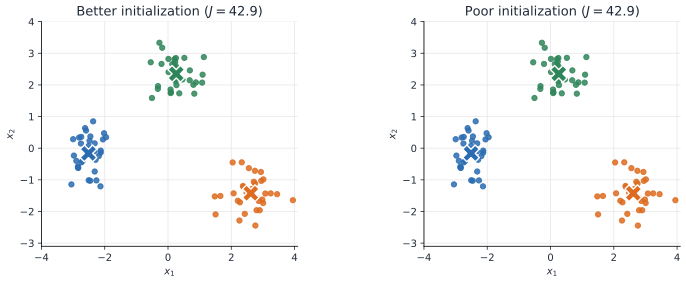
\includegraphics[width=0.86\textwidth]{figures/kmeans/kmeans_initialization_sensitivity.pdf}

\vspace{0.2em}
\begin{itemize}
  \item The objective is not convex in the joint variables $(c,\mu)$.
  \pause
  \item Different initial centroids can lead to different local optima.
  \pause
  \item In practice, use several restarts and keep the smallest final objective.
\end{itemize}
\end{frame}

\begin{frame}{Why Scaling Matters}
\centering
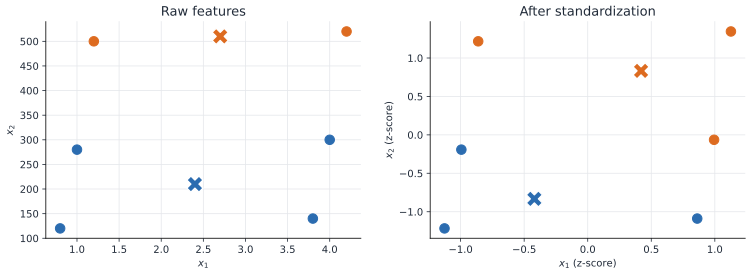
\includegraphics[width=0.92\textwidth]{figures/kmeans/kmeans_scaling_compare.pdf}

\vspace{0.35em}
\begin{itemize}
  \item Since the objective uses squared Euclidean distance, large-scale features can dominate the clustering.
  \pause
  \item This is the same preprocessing issue that already appeared in k-NN.
\end{itemize}
\end{frame}

\begin{frame}{How to Choose $k$}
\centering
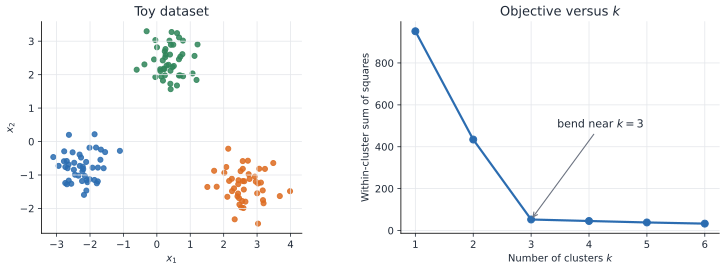
\includegraphics[width=0.92\textwidth]{figures/kmeans/kmeans_elbow_curve.pdf}

\vspace{0.35em}
\begin{itemize}
  \item As $k$ increases, the objective must decrease.
  \pause
  \item The elbow heuristic looks for a visible bend where extra clusters give smaller improvements.
  \pause
  \item This is only a heuristic, not a proof that the chosen $k$ is correct.
\end{itemize}
\end{frame}

\begin{frame}{Relation to PCA}
\begin{columns}[T]
\column{0.5\textwidth}
\textbf{PCA}
\begin{itemize}
  \item optimizes over directions,
  \pause
  \item preserves high-variance structure,
  \pause
  \item outputs coordinates in a lower-dimensional space.
\end{itemize}

\pause
\column{0.5\textwidth}
\textbf{k-means}
\begin{itemize}
  \item optimizes over assignments and centroids,
  \pause
  \item favors compact Euclidean groups,
  \pause
  \item outputs a partition of the dataset.
\end{itemize}
\end{columns}

\pause
\vspace{0.35em}
\footnotesize PCA is often used before k-means for visualization or denoising, but the two objectives are different.
\end{frame}

\begin{frame}{When k-Means Works and When It Fails}
\begin{columns}[T]
\column{0.5\textwidth}
\textbf{k-means often works well when}
\begin{itemize}
  \item clusters are roughly spherical,
  \pause
  \item Euclidean distance reflects similarity,
  \pause
  \item cluster scales are comparable,
  \pause
  \item outliers are limited.
\end{itemize}

\pause
\column{0.5\textwidth}
\textbf{k-means can fail when}
\begin{itemize}
  \item clusters are non-convex,
  \pause
  \item cluster sizes or densities differ strongly,
  \pause
  \item outliers pull centroids away,
  \pause
  \item the representation has poor geometry.
\end{itemize}
\end{columns}
\end{frame}

\begin{frame}{Summary}
\begin{itemize}
  \item k-means minimizes within-cluster squared Euclidean distance.
  \item With fixed centroids, assign each example to the nearest centroid.
  \item With fixed assignments, update each centroid to the cluster mean.
  \item Repeating these two steps gives a simple alternating-optimization method.
  \item The result depends strongly on initialization, scaling, and the choice of $k$.
\end{itemize}
\end{frame}

\begin{frame}{Lab Connection}
\begin{itemize}
  \item Implement the computational core of k-means with NumPy: assignment, centroid update, and objective tracking.
  \item Compare raw features and standardized features.
  \item Project one dataset to 2D with PCA and visualize the cluster assignments there.
  \item Report how initialization and $k$ change the final objective and the qualitative grouping.
\end{itemize}
\end{frame}
